\documentclass[10pt]{article}
\usepackage[polish]{babel}
\usepackage[utf8]{inputenc}
\usepackage[T1]{fontenc}
\usepackage{amsmath}
\usepackage{amsfonts}
\usepackage{amssymb}
\usepackage[version=4]{mhchem}
\usepackage{stmaryrd}
\usepackage{graphicx}
\usepackage[export]{adjustbox}
\graphicspath{ {./images/} }

\title{EGZAMIN WSTĘPNY Z MATEMATYKI }

\author{}
\date{}


\begin{document}
\maketitle
Egzamin składa się z 30 zadań. Zadania 1-10 oceniane będą w skali \(0-2\) punkty, zadania \(11-30\) w skali \(0-4\) punkty. Czas trwania egzaminu - 240 minut.

\section*{Powodzenia!}
\begin{enumerate}
  \item Syn jest o 30 lat młodszy od ojca. 5 lat temu ojciec był 7 razy starszy od syna. W którym roku urodził się syn?
  \item Znaleźć pola kwadratów, których dwoma wierzchołkami są punkty \((-1,1)\) i \((2,1)\).
  \item Podać przykład ciągu niemonotonicznego, którego granicą jest liczba 2.
  \item Dla jakich parametrów \(a\) dziedziną funkcji \(y=\sqrt{a x^{2}+x+a}\) jest zbiór wszystkich liczb rzeczywistych?
  \item Rozwiązać równanie \(\log _{2} x \cdot \log _{x} 4=2\).
  \item Obliczyć sumę współczynników wielomianu \(w(x)=\left(x^{2}+2 x-1\right)^{10}-20 x-3\).
  \item Obliczyć granicę \(\lim _{n \rightarrow \infty} \frac{(n+2)!+n!}{(n+2)!-(n+1)!}\).
  \item Napisać równanie prostej zawierającej tę cięciwę okręgu \(x^{2}-4 x+y^{2}+2 y+1=0\), którą punkt \(A\left(1,-\frac{1}{2}\right)\) dzieli na dwie równe części.
  \item Obliczyć \(f^{\prime}(0)\), jeśli \(f(x)=x(x-1)(x-2)(x-3)(x-4)(x-5)\).
  \item Obliczyć \(\sin \frac{13}{12} \pi\).\\

\includegraphics[max width=\textwidth, center]{2024_11_21_17fc964787b720e2b056g-1}
  \item Znaleźć resztę z dzielenia wielomianu \(x^{1997}-x^{1996}+2\) przez \(x^{3}-x\).
  \item Dla jakiego \(m\) równanie \(\left|x^{2}-2\right|=\log _{\frac{1}{2}} m\) ma dokładnie 4 pierwiastki?
  \item Rozwiązać równanie \(|x-3|^{x^{2}-4 x+3}=1\).
  \item Rozwiązać nierówność \(x+1 \leqslant \sqrt{3+x}\).
  \item Rozwiązać równanie \(\operatorname{tg} x=\operatorname{tg} \frac{1}{x}\).
  \item Niech \(S_{n}\) oznacza sumę \(n\) początkowych wyrazów ciągu \(a_{n}=\frac{2^{n}+3^{n}}{6^{n}}\). Obliczyć \(\lim _{n \rightarrow \infty} S_{n}\).
  \item Ile razy należy rzucić symetryczną monetą, aby z prawdopodobieństwem większym od \(\frac{1}{2}\) otrzymać przynajmniej dwa orły?
  \item Zdarzenia losowe \(A\) i \(B\) są jednakowo prawdopodobne, zawsze zachodzi przynajmniej jedno z nich i \(P(A \mid B)=\frac{1}{2}\). Obliczyć prawdopodobieństwa zdarzeń \(A\) i \(B\). Czy zdarzenia \(A\) i \(B\) są niezależne?
  \item Uzasadnić, że nie istnieje trójkąt o wysokościach długości 1, 2 i 3.
  \item Znaleźć rzut równoległy punktu \(A(5,2,9)\) na płaszczyznę \(O x y\) w kierunku wektora \(\vec{v}=[1,2,3]\).
  \item Rys. 1 przedstawia szkic wykresu funkcji \(f(x)=\frac{a x-b}{x-c}\) dla pewnych liczb \(a, b\) i \(c\). Wyznaczyć współrzędne punktów \(P\) i \(Q\). Wskazać liczby \(a, b\) i \(c\), dla których wykres funkcji \(y=f(x)\) można otrzymać z wykresu funkcji \(y=\frac{1}{x} \mathrm{w}\) wyniku translacji o wektor \(\vec{u}=[1,3]\).\\
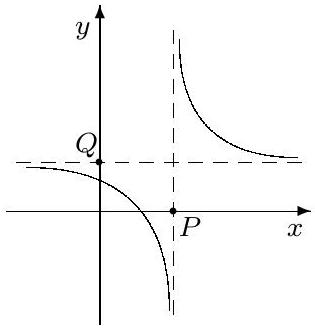
\includegraphics[max width=\textwidth, center]{2024_11_21_17fc964787b720e2b056g-2}
\end{enumerate}

Rys. 1\\
23. Wyznaczyć liczbę \(a\) tak, aby funkcja \(f(x)=\left\{\begin{array}{lll}x^{2}+a x & \text { dla } & x \geqslant 1 \\ \frac{\sin (x-1)}{|x-1|} & \text { dla } & x<1\end{array}\right.\) była ciągła w punkcie \(x_{0}=1\).\\
24. Napisać równanie tej stycznej do wykresu funkcji \(y=\frac{4}{x^{2}}\), która jest nachylona do osi \(O x\) pod kątem \(45^{\circ}\).\\
25. Wyznaczyć przedziały, w których funkcja \(f(x)=2 \cos ^{2} x-x\) jest rosnąca.\\
26. Wyznaczyć asymptoty krzywej \(f(x)=\sqrt{1+x^{2}}-2 x\).\\
27. Przedsiębiorstwo handlowe sprzedaje opony samochodowe. Całkowity zysk przedsiębiorstwa liczony w tysiącach złotych ze sprzedaży \(x\) setek tysięcy opon dany jest wzorem \(z(x)=-x^{3}+9 x^{2}+120 x-400\) dla \(x \geqslant 5\). Przy jakiej ilości sprzedanych opon zysk przedsiębiorstwa będzie największy?\\
28. Punkt \(E\) jest środkiem boku kwadratu \(A B C D\) przedstawionego na rys. 2, a trójkąt \(E F G\) jest równoboczny. Oblicz pole trójkąta \(E F G\), jeżeli długość każdego boku kwadratu \(A B C D\) jest równa 2.\\
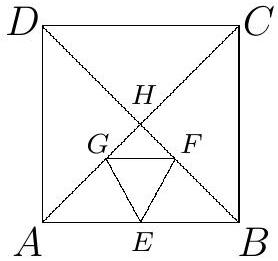
\includegraphics[max width=\textwidth, center]{2024_11_21_17fc964787b720e2b056g-2(1)}

Rys. 2\\
29. Dany jest romb \(A B C D\) o bokach długości 1 i kącie o mierze \(60^{\circ}\) przy wierzchołku \(A\). Obliczyć iloczyn skalarny wektorów \(\overrightarrow{A M}\) i \(\overrightarrow{A N}\), jeśli \(M\) i \(N\) są odpowiednio środkami boków \(B C\) i \(C D\).\\
30. Obliczyć pole powierzchni i objętość wielościanu, którego wierzchołkami są wszystkie środki krawędzi czworościanu foremnego o boku długości \(a\).


\end{document}